\documentclass[12pt,letterpaper,oneside]{report}

% Layout follows Xihong Su's UNH CS dissertation proposal (May 2025):
% title page, Overview chapter, one chapter per work, overall summary chapter, bibliography.
% Preamble and macros are kept in sync with ../thesis/main.tex so chapters can move between the two.

\usepackage[T1]{fontenc}
\usepackage[utf8]{inputenc}
\usepackage[margin=1in,bottom=1.25in,footskip=0.5in]{geometry}
\usepackage[doublespacing]{setspace} % floats and footnotes stay single-spaced
\usepackage{graphicx}
\usepackage[dvipsnames]{xcolor}
\usepackage{booktabs}
\usepackage{microtype}
\usepackage{mathtools,amssymb,amsthm,bm,bbm,amsfonts,nicefrac}
\usepackage{multirow,enumitem}
\usepackage{array}              % column specs like >{\displaystyle}, used by the mprog environment
\usepackage[ruled,linesnumbered,vlined,noend,algosection]{algorithm2e}
\usepackage[american]{babel}
\usepackage[authoryear,round,sort]{natbib}
\let\cite\citep  % \cite gives "(Author, Year)"; use \citet for "Author (Year)"
\usepackage{titlesec}
\usepackage{tikz}
\usepackage{caption}            % For custom caption types, like 'mdp'
\usepackage{thmtools}
\usepackage{thm-restate}
\usepackage{hyperref,url}
\usepackage[noabbrev,capitalize]{cleveref}
\hypersetup{colorlinks=true,citecolor=Blue,linkcolor=black,urlcolor=black}

\usetikzlibrary{automata, positioning, arrows.meta, quotes}
% This creates a new environment called 'mdp' that acts like a figure
\DeclareCaptionType{mdp}[MDP][List of MDPs]
\crefname{mdp}{MDP}{MDPs}
\Crefname{mdp}{MDP}{MDPs}

%%%%%%%%%%%%%%%%%%%%%%%%%%%%%%%%
% PROPOSAL METADATA
%%%%%%%%%%%%%%%%%%%%%%%%%%%%%%%%
\newcommand{\proposaltitle}{Efficient Methods for Risk Aware Decision Making}
\newcommand{\proposalauthor}{Gersi Doko}
\newcommand{\proposaldate}{May, 2026}

\hypersetup{pdftitle={Dissertation Proposal: \proposaltitle},pdfauthor={\proposalauthor}}

%%%%%%%%%%%%%%%%%%%%%%%%%%%%%%%%
% LAYOUT
%%%%%%%%%%%%%%%%%%%%%%%%%%%%%%%%
% "CHAPTER 2" over the centered title
\titleformat{\chapter}[display]
{\normalfont\centering}
{\LARGE\bfseries\MakeUppercase{\chaptertitlename}\ \thechapter}
{1em}
{\Large\bfseries}
\titleformat{name=\chapter,numberless}[block]
{\normalfont\centering\LARGE\bfseries}{}{0pt}{}
\titlespacing*{\chapter}{0pt}{0.5in}{0.5in}

% Operators
\newcommand{\opt}{^{\star}}
\renewcommand{\exp}[1]{\operatorname{exp}\left( #1\right) }
\newcommand{\tr}{^{\mathsf{T}}}
\newcommand{\Real}{\mathbb{R}}
\newcommand{\Nats}{\mathbb{N}}

\DeclareMathOperator{\diag}{diag}

\DeclareMathOperator{\kl}{KL}
\DeclareMathOperator*{\argmin}{arg\,min}
\DeclareMathOperator*{\argmax}{arg\,max}
\DeclarePairedDelimiterXPP\expect[2]{\mathbb{E}_{#1}}[]{}{#2}%
\newcommand{\Ex}[1]{\expect*{}{#1}}
\newcommand{\Exp}[2]{\expect*{#1}{#2}}
\newcommand{\E}[1]{\mathbb{E}\left[\, #1 \,\right]}

% Define risk operators
\newcommand{\risko}{\psi}
\DeclareMathOperator{\varo}{VaR}
\DeclareMathOperator{\cvaro}{CVaR}
\DeclareMathOperator{\conco}{ConC}
\DeclareMathOperator{\oceo}{C}
\DeclareMathOperator{\gento}{GEnT}
\DeclareMathOperator{\fdivo}{FDIV}
\DeclareMathOperator{\evaro}{EVaR}
\DeclareMathOperator{\ermo}{ERM}
\DeclareMathOperator{\ess}{ess}
\DeclareMathOperator{\expectile}{Expectile}
\DeclareMathOperator{\ubsr}{S}

\newcommand{\PiHR}{\Pi_{\mathrm{HR}}}
\newcommand{\PiHD}{\Pi_{\mathrm{HD}}}
\newcommand{\PiAD}{\Pi_{\mathrm{AD}}}
\newcommand{\PiD}{\Pi_{\mathrm{D}}}
\newcommand{\PiR}{\Pi_{\mathrm{R}}}

\newcommand{\Po}{\mathbb{P}}
\renewcommand{\Pr}[1]{\Po\left[ #1 \right]}
\renewcommand{\P}[1]{\Pr{#1}}
\newcommand{\risk}[1]{\psi \left[#1\right]}
\newcommand{\riskd}[2]{\psi_{#1} \left[#2\right]}
\newcommand{\erm}[2]{\ermo_{#1} \left[#2\right]}
\newcommand{\var}[2]{\varo_{#1} \left[#2\right]}
\newcommand{\cvar}[2]{\cvaro_{#1} \left[#2\right]}
\newcommand{\conc}[1]{\conco \left[#1\right]}
\newcommand{\oce}[1]{\oceo \left[#1\right]}
\newcommand{\gent}[2]{\gento_{#1}  \left[#2\right]}
\newcommand{\fdiv}[2]{\fdivo_{#1}  \left[#2\right]}
\newcommand{\evar}[2]{\evaro_{#1} \left[#2\right]}
\newcommand{\ind}[1]{\bm{1}_{#1}}  % Indicator function

\newcommand{\quant}{{\mathfrak{q}}}

% new utility functions
\newcommand{\uvar}{u_{\mathrm{V}}}
\newcommand{\ucvar}{u_{\mathrm{C}}}
\newcommand{\uevar}{u_{\mathrm{E}}}

\DeclareMathOperator{\conv}{cnv}   % convexified function
\DeclareMathOperator{\cl}{cl}      % closure of the function
\newcommand{\conj}{^{\ast}}
\newcommand{\conjconj}{^{\ast\ast}}

% ROIL chapter (from mpemath.sty)
\newcommand{\eps}{\varepsilon}
\DeclareMathOperator{\ext}{ext}   % extreme points
\newcommand{\subjectto}{\operatorname{subject\, to} &}
\newcommand{\minimize}[1]{\operatorname*{minimize}_{#1} &}
\newcommand{\maximize}[1]{\operatorname*{maximize}_{#1} &}
\newenvironment{mprog}{
\begin{array}{>{\displaystyle}c>{\displaystyle}l>{\displaystyle}l}}{
\end{array}}
\newcommand{\stc}{\\[1ex] \subjectto}
\newcommand{\cs}{\\[1ex] & }

% fast-risk chapter (from fastcvar/main.tex and its mpemath.sty)
\DeclareMathOperator{\ER}{DR}
\DeclareMathOperator{\qvar}{QuickVaR}
\DeclareMathOperator{\ews}{EWS}
\DeclareMathOperator{\tvaro}{TVaR}
\newcommand{\tvar}[2]{\tvaro_{#1} \left[#2\right]}
\SetKwInOut{Input}{Input}
\SetKwInOut{Output}{Output}
\IncMargin{2em}

%%%%%%%%%%%%%%%%%%%%%%%%%%%%%%%%
% THEOREMS
%%%%%%%%%%%%%%%%%%%%%%%%%%%%%%%%
\theoremstyle{plain}
\newtheorem{theorem}{Theorem}[section]
\newtheorem{proposition}[theorem]{Proposition}
\newtheorem{lemma}[theorem]{Lemma}
\newtheorem{corollary}[theorem]{Corollary}
\theoremstyle{definition}
\newtheorem{definition}[theorem]{Definition}
\newtheorem{assumption}[theorem]{Assumption}
\theoremstyle{remark}
\newtheorem{remark}[theorem]{Remark}
\newtheorem{example}[theorem]{Example}

% -- comment commands
\newcommand{\mm}[1]{\textcolor{red}{(MP:\ #1)}}
\newcommand{\gersi}[1]{\textcolor{blue}{(GD:\ #1)}}
\newcommand{\todo}[1]{\textcolor{orange}{(TODO:\ #1)}}
\newcommand{\cc}{\bgroup\color{ForestGreen}\let\ccnext=}

\begin{document}

%%%%%%%%%%%%%%%%%%%%%%%%%%%%%%%%
% TITLE PAGE
%%%%%%%%%%%%%%%%%%%%%%%%%%%%%%%%
\begin{titlepage}
  \centering
  \singlespacing
  \vspace*{1.5in}
  Dissertation Proposal\\
  \proposaltitle\par
  \vfill
  \proposalauthor\par
  \bigskip
  University of New Hampshire\par
  Department of Computer Science\par
  \vfill
  \proposaldate\par
  \vspace*{1in}
\end{titlepage}

% \tableofcontents % not in the reference proposal; uncomment if wanted

%%%%%%%%%%%%%%%%%%%%%%%%%%%%%%%%
% TEXT
%%%%%%%%%%%%%%%%%%%%%%%%%%%%%%%%
\setcounter{page}{1}

%%%%%%%%%%%%%%%%%%%%%%%%%%%%%%%%
\chapter{Overview}\label{ch:overview}

\section{Introduction}\label{sec:overview-intro}

% ported verbatim from ../thesis/chapters/introduction.tex
The field of machine learning studies and develops algorithms that can perform tasks without being explicitly programmed to do so. Reinforcement learning(RL) is a subfield of machine learning that studies how machines may be trained to perform well in environments they were not explicitly programmed to operate in~\citet{Sutton1998}. This process is summarized typically in a ``loop'' of observing the state of a system, taking an action, and receiving a reward. The objective the RL process is to learn a \emph{policy} which maps states to actions in a way that maximizes the expected sum of rewards over time.

When making decisions in real life we often stop and consider possible outcomes of our actions. We evaluate the future state of the world if we were to take that action, and we may consider many possible actions this way. After evaluation the possible actions and their outcomes, we then take the action which corresponds with the best outcome. This process of evaluating the future possible states of the world and making decisions which maximize those future values is exactly the core of RL.

The outcomes of actions in the real world is uncertain. The same action can have different effects depending on the environment. As a result this notition of maximizing future reward needs to have a method of evaluating the value of future random outcomes. Traditionally, RL algorithms maximize the expected value of the return, which is the sum of all possible future outcomes multiplied by their probability of occuring. This is often seen in games of chance when evaluating the expected value of a bet or random outcome.

The expected value, while a useful metric has its downsides. For example consider flipping a fair coin. If heads you win and I pay you 1\$, if tails you lose and you pay me 1\$. The expected value of this bet is 0\$, but consider the same betting scheme where instead of losing or gaining 1\$ you lose or gain 100\$. The expected value is still 0\$, but many of us would consider the latter bet to be much riskier. More generally, expected value ignores the distribution of outcomes and only considers their avereage. In real world applications such as medicine, agriculture, finance, and robotics we often care about events that are unlikely to occur, but catastrophic if they do. In these cases we want to follow the same scheme as in traditional RL, but instead of computing value from expecation, we compute value from something called a \emph{risk measure}.

Risk measures come in many variations~\cite{Follmer2016, rockafellar2002conditional, Shapiro2017}. Some risk measures exhibit properties that may be desireable to a particular application while others may not. For example in when making decisions in medicine we may want to consider the worst case scenario of a treatment, while in finance we may want to consider the average of the worst 5\% of outcomes.

The field of risk sensitive reinforcement learning has developed methods for optimizing these risk measures in the context of RL~\cite{Chow2015, chavez2026sample, Bauerle2011}. This work is a continuation of this line of research. Our objective is to efficiently and effectively optimize risk measures in the context of RL to obtain risk aware policies we can deploy in fields like healthcare, agriculture, finance, and robotics.

In this work we will primarily focus on specific contributions to the field of risk aware reinforcement learning. Broadly our contributions here are threefold. First we develop a method for robustly learning policies from demonstrations in an offline setting. Second we develop algorithms for computing risk measures in linear time. Finally we develop the notion of extended time consistent risk measures, their properties, limitations, and their relationship with prior works.

\section{Overview of Dissertation}\label{sec:overview-outline}

This proposal is organized as follows. \Cref{ch:roil} presents our work on robust offline imitation learning. This work most broadly answers the question of how to learn a polciy from a dataset of demonstrations which will robustly generalize to the environment. The notion of robustness that is considered in \Cref{ch:roil} resembles a worst case adversarial outcome which we contrast with existing immitation learning techniques. \Cref{ch:fast-risk} demonstrates our novel contributions to computing monetary risk measures in linear time. Our algorithm enjoys near order of magnitude speedups in computing these risk measures and is implemented in a julia repo for the public \url{https://github.com/RiskAverseRL/RiskMeasures.jl}. Finally, \Cref{ch:etc} presents our work on extended time consistent risk measures in MDPs. We first illustrate what properties these risk measure have and how they are desireable to modern RL practitioners. Then we describe existing risk measures, where they fall short of these properties, and what results that can have when solving related MDPs. \Cref{ch:contributions} summarizes the contributions of this dissertation and outlines future work.

%%%%%%%%%%%%%%%%%%%%%%%%%%%%%%%%
\chapter{Robust Offline Imitation Learning}\label{ch:roil}

% chapter summary: paper abstract, verbatim from ../thesis/chapters/roil.tex
We study the problem of imitation learning via inverse reinforcement learning where the agent attempts to learn an expert's policy from a dataset of collected state, action tuples. We derive a new Robust model-based Offline Imitation Learning method (ROIL) that mitigates covariate shift by avoiding estimating the expert's occupancy frequency. Frequently in offline settings, there is insufficient data to reliably estimate the expert's occupancy frequency and this leads to models that do not generalize well. Our proposed approach, ROIL, is a method that is guaranteed to recover the expert's occupancy frequency and is efficiently solvable as an LP. We demonstrate ROIL's ability to achieve minimal regret in large environments under covariate shift, such as when the state visitation frequency of the demonstrations does not come from the expert.

\paragraph{Publications} \todo{venue and full citation}

\section{Introduction}\label{sec:roil-intro}

\todo{}

\section{Previous Work}\label{sec:roil-prior}

\todo{}

\section{Our Work}\label{sec:roil-ours}

\todo{}

\section{Experiments}\label{sec:roil-experiments}

\todo{}

\section{Conclusion}\label{sec:roil-conclusion}

\todo{}

%%%%%%%%%%%%%%%%%%%%%%%%%%%%%%%%
\chapter{Computing Monetary Risk Measures in Linear Time}\label{ch:fast-risk}

% chapter summary: paper abstract, verbatim from ../thesis/chapters/fast-risk.tex
Monetary risk measures have gained popularity for expressing decision-makers' risk aversion. Value-at-Risk (VaR) and Conditional-Value-at-Risk (CVaR), in particular, are used commonly for this purpose. This chapter proposes new efficient algorithms to compute these risk measures for a discrete random variable in expected linear time with respect to the size of its domain. First, we propose QuickVaR, an algorithm that computes the VaR of a discrete random variable. Then, we leverage QuickVaR to propose QuickDivergence, an algorithm for computing a class of $\varphi$-divergence risk measures, including the popular CVaR risk measure. The QuickVaR algorithm adapts the well-known quickselect algorithm, while QuickDivergence builds on polymatroid optimization algorithms. Numerical results show that our new algorithms offer speedups of up to nearly an order of magnitude for large domains. A library implementation is available at \url{https://github.com/RiskAverseRL/RiskMeasures.jl}.

\paragraph{Publications} \todo{venue and full citation}

\section{Introduction}\label{sec:fast-risk-intro}

\todo{}

\section{Previous Work}\label{sec:fast-risk-prior}

\todo{}

\section{Our Work}\label{sec:fast-risk-ours}

\todo{}

\section{Experiments}\label{sec:fast-risk-experiments}

\todo{}

\section{Conclusion}\label{sec:fast-risk-conclusion}

\todo{}

%%%%%%%%%%%%%%%%%%%%%%%%%%%%%%%%
\chapter{Extended Time Consistent Risk Measures in MDPs}\label{ch:etc}

% chapter summary: paper abstract, verbatim from ~/grad/primal/cvar.tex (draft; re-sync if it changes)
Risk-averse Markov decision processes (MDPs) optimize a risk measure of the return, and their optimal policies typically depend on a risk level that the agent updates along its trajectory. We study whether such updates can always preserve optimality: does there always exist a way to update the risk level such that an optimal policy will remain optimal? We formalize this property as \emph{extended time consistency} (ETC) and study it for two broad classes of risk measures. For utility-based shortfall risk measures, including value-at-risk (VaR), the entropic risk measure, and expectiles, we prove that ETC holds and derive an exact dynamic program over the risk level. For optimized certainty equivalents, we show that the conditional value-at-risk (CVaR) is not ETC. Our analysis rests on a duality between disutility-based and risk-level dynamic programs.

\paragraph{Publications} This work is in progress and has not yet been published.

\section{Introduction}\label{sec:etc-intro}

\todo{}

\section{Previous Work}\label{sec:etc-prior}

\todo{}

\section{Our Work}\label{sec:etc-ours}

\todo{}

\section{Experiments}\label{sec:etc-experiments}

\todo{}

\section{Conclusion}\label{sec:etc-conclusion}

\todo{}

%%%%%%%%%%%%%%%%%%%%%%%%%%%%%%%%
\chapter{Summary of Contributions}\label{ch:contributions}

Figure \ref{fig:overview} illustrates the overall concrete deliverables for the result of this proposal. Firstly we develop ROIL, an offline method for robustly recovering expert policies from demonstrations in an adversarial manner. Secondly we develop QuickVaR and QuickDivergence, two algorithms for computing monetary risk measures in linear time which improves on traditional approaches by a log factor. Finally we develop the notion of extended time consistent risk measures in MDPs, why they are important, what existing measures satisfy this property, and how to solve the RL problem given these measures of risk.

\begin{figure}[ht]
  \centering
  % \includegraphics[width=\textwidth]{figs/overview}
  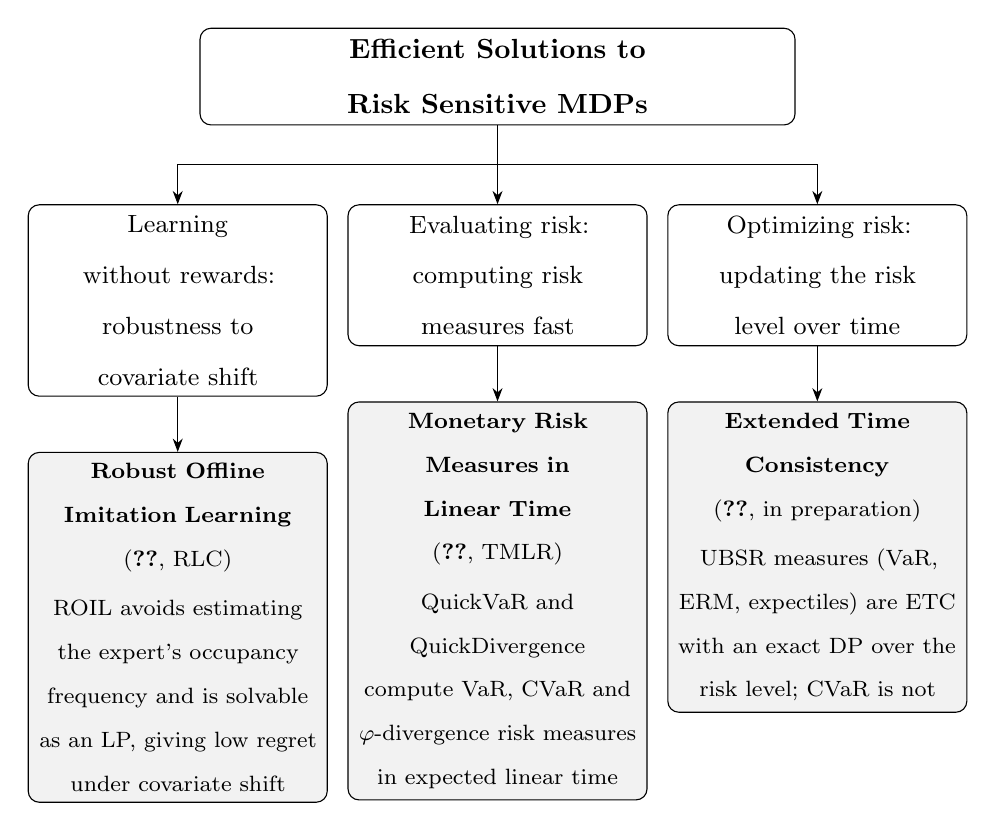
\begin{tikzpicture}[
      box/.style={draw, rounded corners, align=center, inner sep=4pt, execute at begin node={\hyphenpenalty=10000\exhyphenpenalty=10000}},
      root/.style={box, text width=0.6\textwidth, font=\bfseries},
      theme/.style={box, text width=0.29\textwidth, minimum height=1.75cm, font=\small},
      paper/.style={box, text width=0.29\textwidth, minimum height=3.7cm, font=\footnotesize, fill=gray!10},
      edge/.style={-{Stealth}},
    ]
    \node[root] (root) {Efficient Solutions to Risk Sensitive MDPs};

    \node[theme, anchor=north] (t2) at ([yshift=-1cm]root.south) {Evaluating risk:\\ computing risk measures fast};
    \node[theme, anchor=north east] (t1) at ([xshift=-0.25cm]t2.north west) {Learning without rewards:\\ robustness to covariate shift};
    \node[theme, anchor=north west] (t3) at ([xshift=0.25cm]t2.north east) {Optimizing risk:\\ updating the risk level over time};

    \node[paper, anchor=north] (p1) at ([yshift=-0.7cm]t1.south) {\textbf{Robust Offline Imitation Learning}\\ (\cref{ch:roil}, RLC)\\[2pt] ROIL avoids estimating the expert's occupancy frequency and is solvable as an LP, giving low regret under covariate shift};
    \node[paper, anchor=north] (p2) at ([yshift=-0.7cm]t2.south) {\textbf{Monetary Risk Measures in Linear Time}\\ (\cref{ch:fast-risk}, TMLR)\\[2pt] QuickVaR and QuickDivergence compute VaR, CVaR and $\varphi$-divergence risk measures in expected linear time};
    \node[paper, anchor=north] (p3) at ([yshift=-0.7cm]t3.south) {\textbf{Extended Time Consistency}\\ (\cref{ch:etc}, in preparation)\\[2pt] UBSR measures (VaR, ERM, expectiles) are ETC with an exact DP over the risk level; CVaR is not};

    \foreach \t in {t1, t2, t3} {\draw[edge] (root.south) -- ++(0,-0.5cm) -| (\t.north);}
    \draw[edge] (t1) -- (p1);
    \draw[edge] (t2) -- (p2);
    \draw[edge] (t3) -- (p3);
  \end{tikzpicture}
  \caption{Overview of the dissertation.}\label{fig:overview}
\end{figure}

%%%%%%%%%%%%%%%%%%%%%%%%%%%%%%%%

\begingroup
\singlespacing
\setlength{\bibsep}{\baselineskip}
\bibliographystyle{apalike}
\bibliography{proposal}
\endgroup

\end{document}
